%!TEX program = xelatex
% Note: this template must be compiled with XeLaTeX rather than PDFLaTeX
% due to the custom fonts used. The line above should ensure this happens
% automatically, but if it doesn't, your LaTeX editor should have a simple toggle
% to switch to using XeLaTeX.

\documentclass[
	aspectratio=169, % Uncomment to use an aspect ratio of 16:9 (160 mm by 90 mm)
	%aspectratio=43, % Uncomment to use an aspect ratio of 4:3 (128mm by 96mm)
	t, % Top align all slide content by default
	onlytextwidth, % Typeset content in columns at text width
	10pt, % Default font size, use 10pt for the 16:9 aspect ratio and 8pt for the 4:3 aspect ratio
]{beamer}

\usepackage{../ImperialTheme/beamerthemeImperial} % Use the Imperial theme

\def\imagefolder{../ImperialTheme/Images/}

\title{A modification of the mesh} % Presentation title to appear on the title slide and left footers

\subtitle{} % Presentation subtitle to appear on the title slide

\author{Víctor Ballester} % Author name(s) to appear on the title slide

\date{\today} % Presentation date to appear on the title slide and right footers

\begin{document}

\begingroup
\setbeamercolor{background canvas}{bg=ICLBlue} % Slide background color
\setbeamercolor{title page title}{fg=white} % Title text color
\setbeamercolor{title page subtitle}{fg=white} % Subtitle text color
\setbeamercolor{author}{fg=white} % Author(s) text color
\setbeamercolor{date}{fg=white} % Date text color
\setbeamertemplate{title page}[logo]{\imagefolder/ICL_Logo_White.pdf} % Imperial logo color, use 'ICL_Logo_White.pdf' for white and 'ICL_Logo_Blue.pdf' for blue
\frame[plain, s]{\titlepage} % Output the title page with no footer ('plain') and vertically distributed text ('s')
\endgroup

\begin{frame}
	\frametitle{New domain}
	\begin{columns}[T] % [T] ensures correct vertical alignment
	\begin{column}{0.38\linewidth} % Left column
		\begin{itemize}
			\item Points on the quads edges at different geometric progressions.
			\item \textbf{Aim:} ``homogenize" the CFL condition through the domain, in this case by increasing the size of the first triangles.
			\item So far: $dt_\text{old} \sim 0.0012\implies dt_\text{new} \sim 0.003$
		\end{itemize}
	\end{column}
	\begin{column}{0.58\linewidth} % Right column
		{
			\centering
			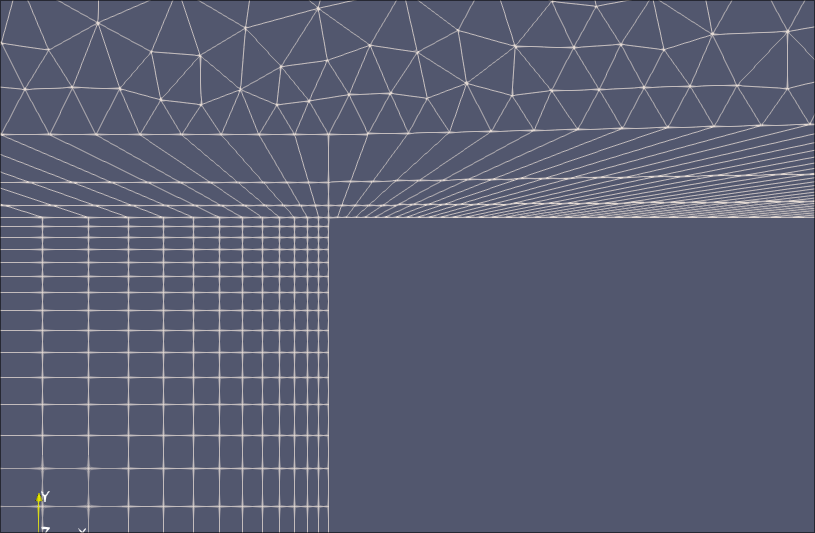
\includegraphics[width=\linewidth]{Images/zoomeddomain.png}
		}
	\end{column}
	\end{columns}
	
        
\end{frame}
\begin{frame}
	\frametitle{New domain}

  \begin{itemize}
		\item Boundary layer of quads also changed. Now its height increases with $x$.
		\item \textbf{Aim 1:} take advantage of the efficiency of quads integration and mirror the boundary layer growth
		\item \textbf{Aim 2:} have similar aspect ratios sizes at the outflow to match triangles sizes (in order to avoid jumps). Because the mesh at the outflow is very sparse.
	\end{itemize}

	{
	\centering
	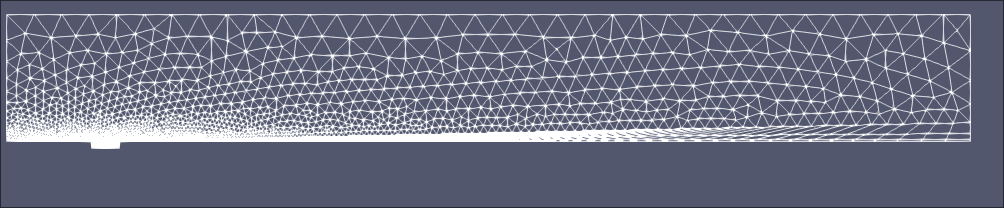
\includegraphics[width=\linewidth]{Images/domain.png}
	}

	
\end{frame}
\begin{frame}
	\frametitle{TS waves!!!}
	
	\begin{itemize}
		\item New width considered, $w=16.35 \delta^*$, which doesn't have global instability. (Reminder: we already know that $w=16.5 \delta^*$ has an global instability).
	\end{itemize}

	{
	\centering
	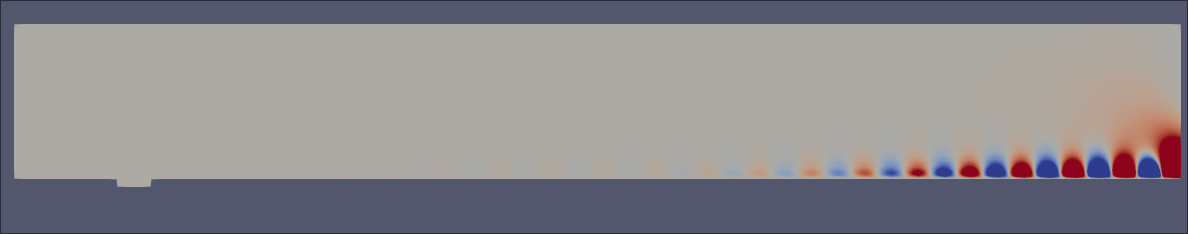
\includegraphics[width=\linewidth]{Images/v_TS.png}
	$v$ component of the most unstable mode.
	}

\end{frame}
\begin{frame}
	\frametitle{Some problems}

	\begin{itemize}
		\item Sheared boundary layer. Probably because I am keeping the same polynomial order of approximation on the quads, but one of the dimensions is changing (stretching) \textbf{a lot} (see figures below).
		\item Post-processing improves something, but we need to modify the integration as well.
	\end{itemize}
	
	{
	\centering
	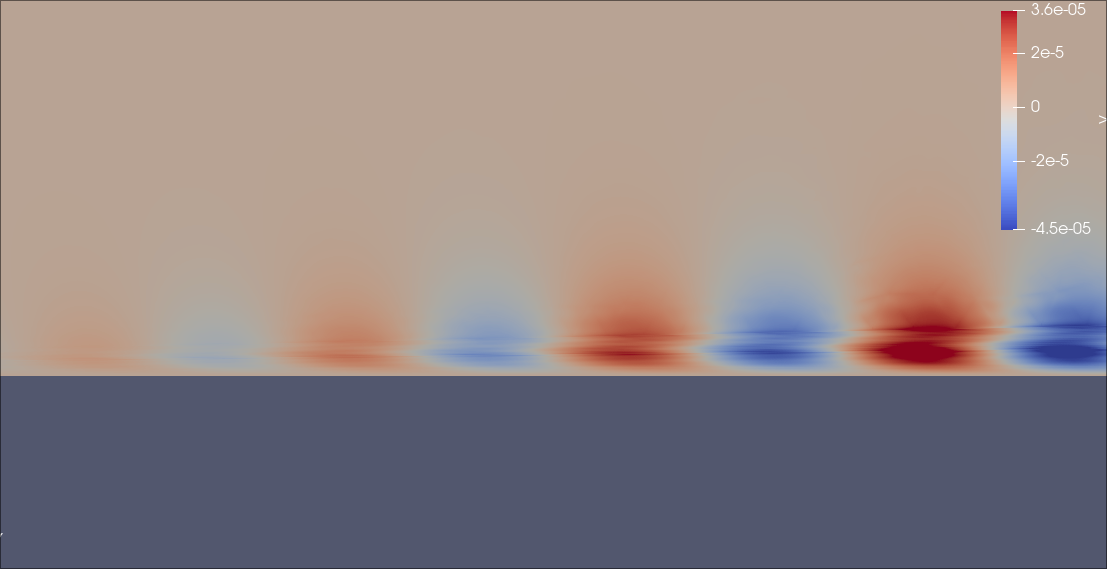
\includegraphics[width=\linewidth]{Images/shear_nozoom.png}
	}


\end{frame}
\begin{frame}
	\frametitle{Some problems}
	
	{
	\centering
	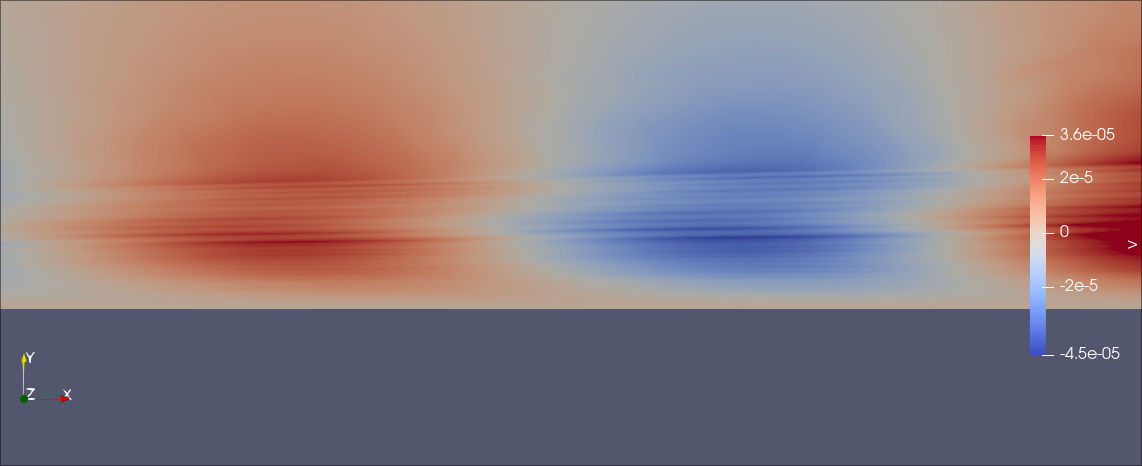
\includegraphics[width=\linewidth]{Images/shear.png}
	}
\end{frame}
\begin{frame}
	\frametitle{Some problems}
	
	{
	\centering
	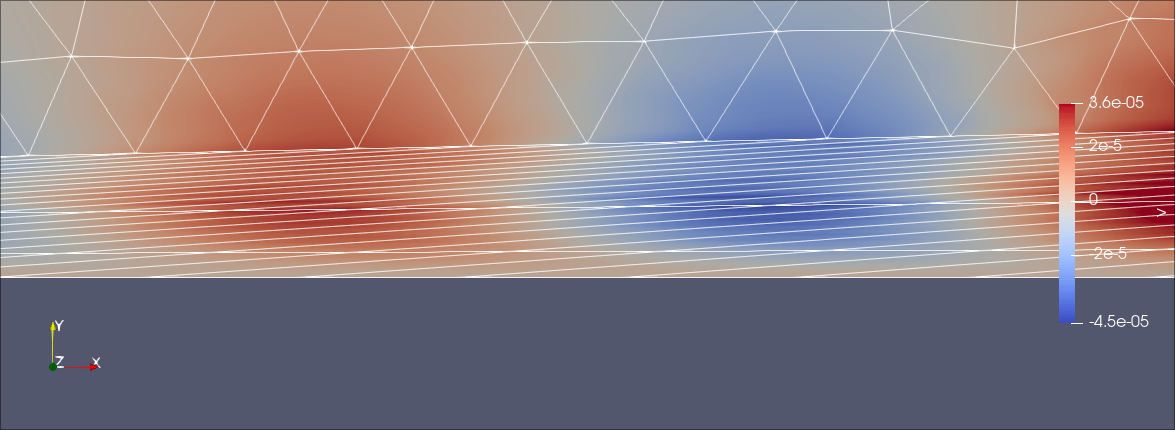
\includegraphics[width=\linewidth]{Images/shear_mesh.png}
	}
\end{frame}
\end{document}
